\section{Requirement Engineering}

\subsection{Definition}

Before the definition, we give a possible scenario to understand what requirement engineering is.

\highspace
The municipality of Milan says the following: \dquotes{\emph{The time it takes to make decisions on building permits for residential buildings in the city is too long. We want to develop software that will help us reduce this time}}. So where do we start? How do we identify the most important aspects? How do we make sure that we have understood what our customers want from us?

\begin{definitionbox}
    Software measure engineering (\definition{Requirement Engineering}) is the process of discovering the purpose for which the software is intended by identifying stakeholders and their needs, and documenting these in a form suitable for analysis, communication and subsequent implementation.
\end{definitionbox}

\noindent
The questions derived from requirements engineering are:
\begin{itemize}
    \item Identify stakeholders
    \item Identify their needs
    \item Produce documentation
    \item Analyze, communicate, implement requirements
\end{itemize}

\begin{figure}[!htp]
    \centering
    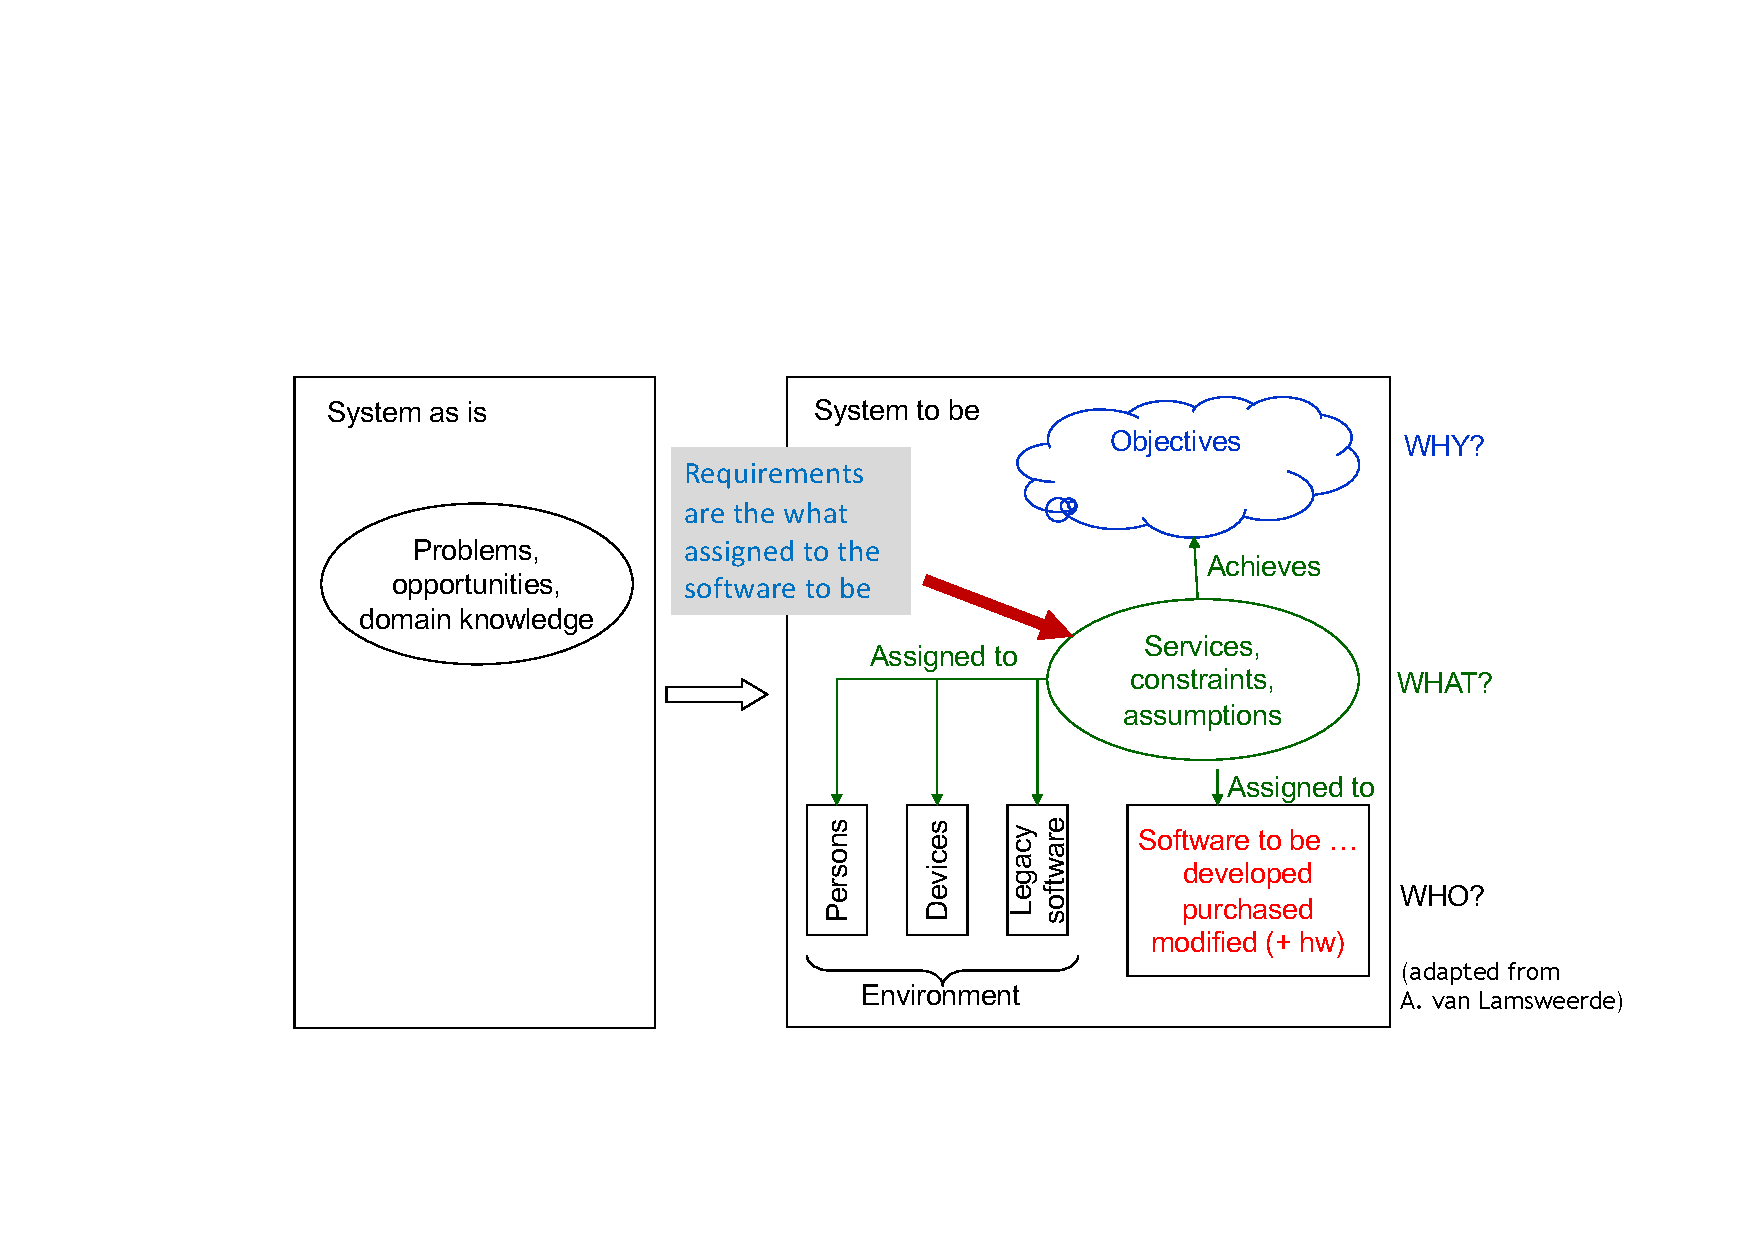
\includegraphics[width=\textwidth]{img/requirement-engineering-1.pdf}
    \caption{Analyzing the system as is and the system to be.}
\end{figure}